% !TeX root = skripta-konstitutivni-vztahy-materialu.tex
% !TeX lastmodified = 2019-11-19

\subsection{Shear}
Jak \uv{simple shear}, tak \uv{pure shear} je zvykem používat ve smyslu deformace. Oba stavy deformace jsou teoreticky ekvivalentní, v~praxi tomu však tak nemusí být (není snadné pro obecný Poissonův poměr $\mu$ realizovat příslušné stavy deformace, pro $\mu = \num{0.5}$ je to snazší).

\subsubsection{Simple shear}
\begin{figure}[H]
	\centering
	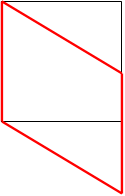
\includegraphics[height=4cm]{simple-shear}
	\caption{Simple shear}
	\label{fig:simple-shear}
\end{figure}

\begin{itemize}
	\item černá je nedeformovaná geometrie
	\item červená je deformovaná geometrie
	\item třetí rozměr zůstává bez změny ($\lambda_3 = 1$)
	\item volumetrická změna $= 0$
	\item pozor: indukují se i normálová napětí (při velkých -- \uv{neinfinitezimálních} -- deformacích)
	\item hlavní osy tenzoru deformace se v průběhu vzrůstající úrovně deformace NATÁČEJÍ
\end{itemize}

Praktická realizace:
\begin{figure}[H]
	\centering
	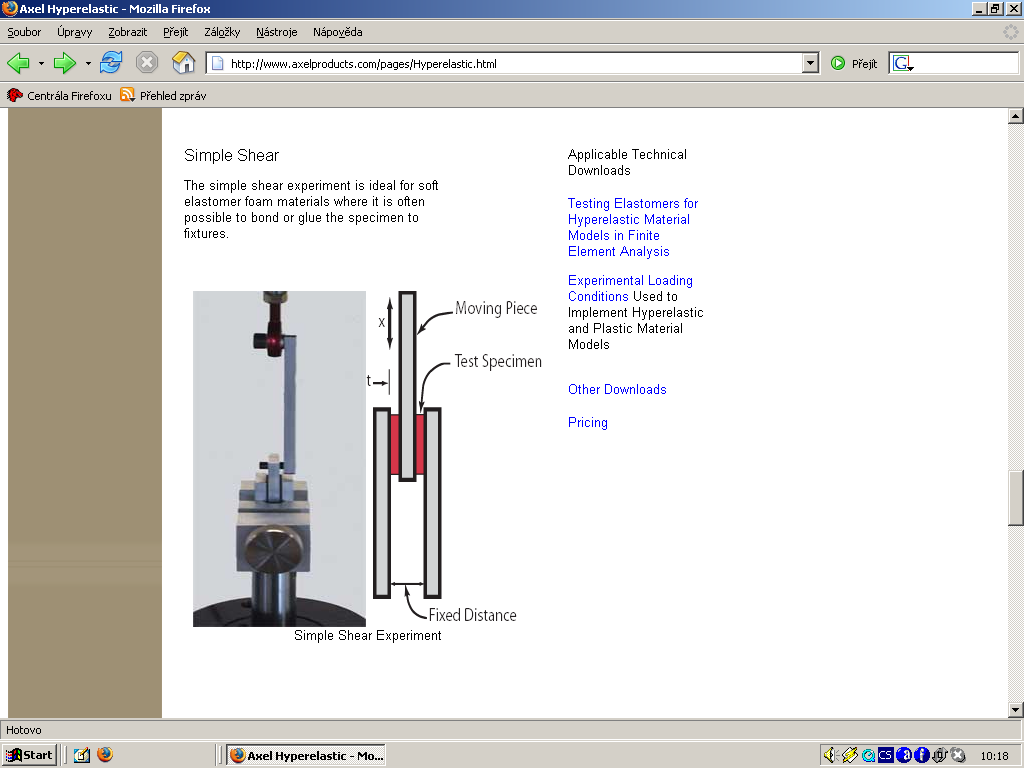
\includegraphics[width=0.4\linewidth]{Obrazky/simple-shear-experiment}
	\caption{Simple shear experiment}
	\label{fig:simple-shear-experiment}
\end{figure}
Test je vhodný pro poddajné pěnové materiály, u~nichž nelze realizovat ekvivalenty čistého smyku v~rovinné deformaci.

\subsubsection{Pure shear}
\begin{figure}[H]
	\centering
	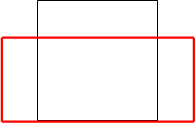
\includegraphics[height=4cm]{pure-shear}
	\caption{Pure shear}
	\label{fig:pure-shear}
\end{figure}

\begin{itemize}
	\item třetí rozměr zůstává bez změny ($\lambda_3 = 1$)
	\item volumetrická změna $= 0$ (v~praxi při tzv. \uv{pure shear} testu není většinou splněno)
	\item praktická realizace: tahem v~širokých čelistech na širokém vzorku nebo tlakem hranolového vzorku při zabránění jedné z~příčných deformací
\item hlavní osy deformace se v~průběhu vzrůstající úrovně deformace nenatáčí
\end{itemize}

\subsubsection{Vysvětlení vzájemné ekvivalence obou testů}
\begin{figure}[H]
	\centering
	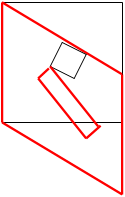
\includegraphics[height=4cm]{shear-vzajemna-ekvivalence}
	\caption{Vzajemná ekvivalence}
	\label{fig:shear-vzajemna-ekvivalence}
\end{figure}

Na případu \enquote{simple shear} lze pro danou úroveň deformace (gama) vždy nalézt na deformovaném vzorku ortogonální (pravoúhlý) element, kterému v nedeformované konfiguraci odpovídá rovněž ortogonální element. Tedy na takovém elementu neproběhl smyk vůči jeho hranám -- element se pouze cely natočil, v jednom směru natáhl a~v~druhém stlačil (volumetrická změna $= 0$). Stav deformace pro tento element je z~podstaty věci ekvivalentní stavu \enquote{pure shear}. Jediný rozdíl je v~NATÁČENÍ hlavních os deformace,  proto také zápis obou typů deformací do podoby deformačního gradientu je vzájemně odlišný -- deformační gradient obsahuje totiž i~rotaci tělesa („rigid body rotation“).

\begin{figure}[H]
	\centering
%	\includegraphics[height=4cm]{}
	\caption{Možné rozpory při záměně ekvivalentů smykové napjatosti}
%	\label{fig:}
\end{figure}

